% - Multi-object tracking problem, assumptions
%     - Recall some part from Intro, gradually from JPDA to PHD
% - Object birth/survival

In this section, we provide the theoretical background of the multi-target tracking problem. We have already established the foundations of Bayesian filtering and explained in detail how the Kalman filter works. Now, we will discuss how it differs from other filters that are used for tracking objects. Before we start building the theoretical foundations for object tracking filters, we need to clarify the difference between Bayesian filtering and Bayesian object tracking.

When we track objects, we rely on measurements from sensors, such as cameras, lidars, or radars. These sensors have specific technical specifications and limitations, and there is no sensor that can be 100\% reliable. The reliability of a sensor may be affected by noise, which occurs when a sensor detects an object that is not present. This behavior may be caused by weather conditions in the sensor's operating area, the sensor's limited resolution, or dirt or dust covering the sensor's surface. We do not address the exact reasons why this happens; we only need to find ways to eliminate noisy measurements and separate them from measurements generated by existing objects.

The second problem is closely related to the first. It occurs when a sensor fails to generate measurements for objects that are present in its field of view. The reasons for this may be the same as for noisy measurements, and we do not address these reasons directly. However, we must be able to mathematically model these situations to ensure that they can be properly handled by the filter we want to use to track objects.

These two problems have their names that we will use in this work. Noisy measurements are called \textit{clutter}, and missing measurements are called \textit{misdetections}. We have already seen that the latter problem can be handled by the Kalman filter by skipping the update step. Clutter, on the other hand, creates a much more challenging problem. Figure \ref{fig:clutter-intro} shows what clutter looks like to the filter. In the left image, we see a track of an object and measurements generated by the sensor, shown in red. Clutter measurements are shown as blue asterisks. We can distinguish between measurements and clutter. However, in the right image, we see how the filter sees the same data points, with all points in the same color. To the filter, all these points look the same, and there is no easy way to distinguish between clutter and real measurements.

\begin{figure}
\centering
\begin{subfigure}[t]{.45\textwidth}
  \centering
  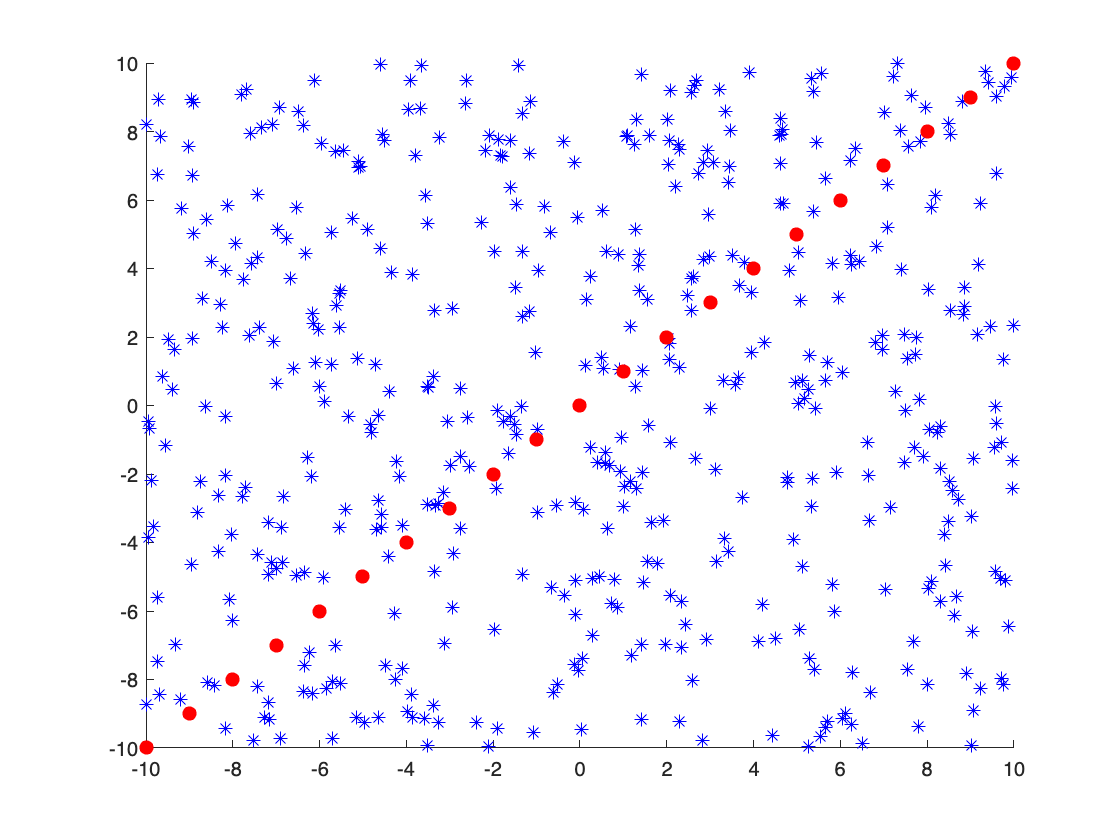
\includegraphics[width=.9\linewidth]{figures/clutter.intro.1.png}
   \caption{Real measurements from some object are shown as red dots. Clutter measurements are displayed as blue asterisks.}
  \label{fig:clutter-intro:1}
\end{subfigure}\hfill
\begin{subfigure}[t]{.45\textwidth}
  \centering
  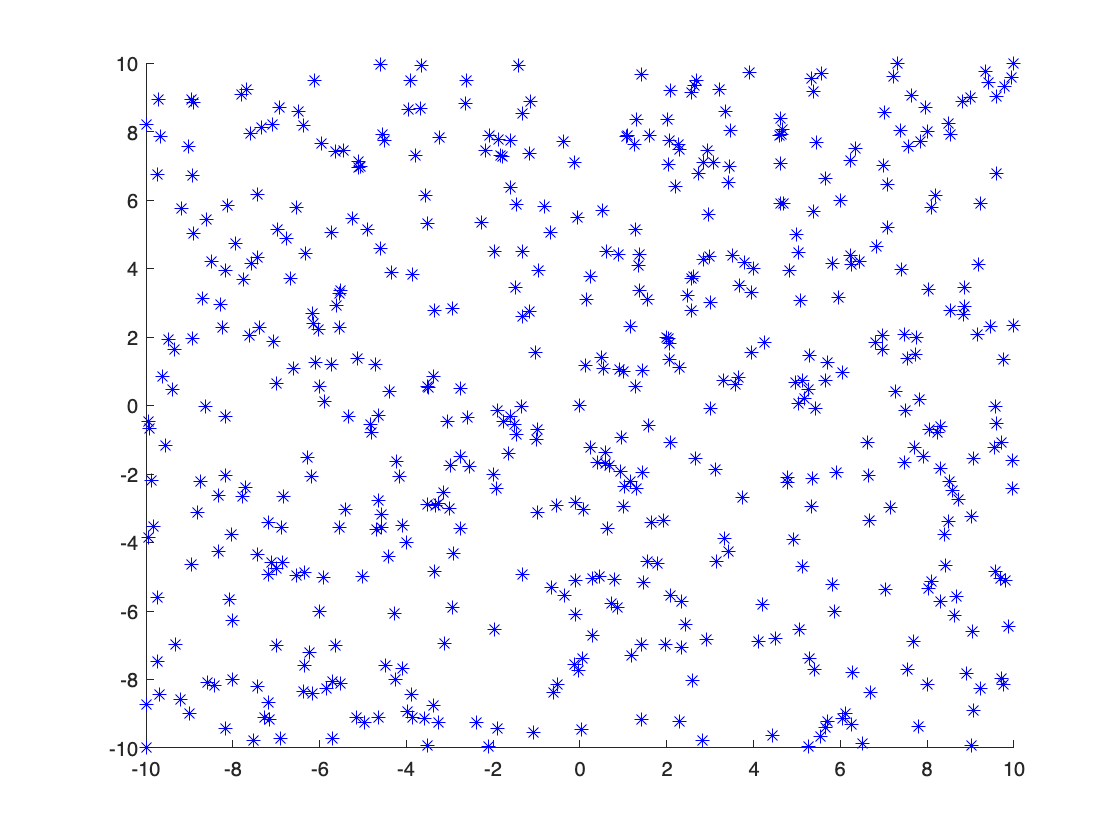
\includegraphics[width=.9\linewidth]{figures/clutter.intro.2.png}
  \caption{Both real measurements and clutter measurements are shown as blue asterisks.}
  \label{fig:clutter-intro:2}
\end{subfigure}
\caption{Measurements in clutter. In this Figure, we indicate the clutter problem. When a sensor generates measurements, some of them may be clutter measurements, and there is no easy way to distinguish which data points come from a real object and which are noise.}
\label{fig:clutter-intro}
\end{figure}

The uncertainty in distinguishing between real measurements and clutter has led to the development of many methods for addressing this problem. The main idea behind these methods is that, since we have no information about which measurements come from targets and which are clutter, we should consider all measurements at each time step as coming from a target. This involves creating all possible assignments between measurements and targets and then evaluating the probability of each such assignment. In other words, we evaluate the possibility that a given measurement comes from a specific target according to its motion model. If the measurement is too far from the target, the probability of such an assignment will be lower than that of an assignment with a measurement that is close to the predicted state. These assignments are referred to as \textit{association hypotheses}. In the following subsection, we will provide a brief overview of various target tracking methods and approaches. But before doing so, we will outline the main assumptions of multi-target tracking (MTT).

\subsection{Overview of target tracking methods}

There are multiple filters that use association hypotheses. For single-target tracking, when the maximum number of targets is fixed to one, in Gaussian-linear scenarios the Probabilistic Data Association (PDA) filter can be utilized \cite{bar-shalomProbabilisticDataAssociation2009}. At each time step, this filter creates new hypotheses for all possible data associations and creates a joint posterior distribution after at the update step. Each hypothesis is assigned with a weight that reflects the likelihood that it actually originates from the target. Next, the resulting Gaussian mixture is reduced to only one Gaussian that represents the posterior state of the target. Both Gaussian mixtures and the reduction techniques will will be discussed later in this work.

This PDA filter is conceptually very simple and straightforward, but it may be too simple for many real-world scenarios, particularly when there are multiple targets present that are too close to each other to be tracked by multiple instance of the PDA filter. This is addressed in the extension and the resulting filter is named the Joint Probabilistic Data Association (JPDA) filter \cite{bar-shalomMultitargetmultisensorTrackingPrinciples1995}. It can handle multiple targets all at once but only when the number of targets is known in advance. The main idea behind this filter is that at each time step it creates all possible measurement-to-target association hypotheses, and, for each target, it creates a joint probability from all partial probabilities computed for each measurement. The series of such probabilities create tracks, and the track with the highest probability is considered the real track of the object. Because of the way how hypotheses are calculated, the JPDA filter is computationally much more expensive than the PDA filter. Moreover, if tracks get too close to each other, this filter shows the problem called the track coalescence—when tracks of two targets merge into one track.

Both PDA and JPDA filters are single-scan methods, which means they process only one set of measurements at a time. Compared to single-scan methods, there exist multi-scan methods that compute probabilities of tracks based on the history of all measurements, in a hierarchical manner. This way of calculating posterior probabilities leads to significant improvements in tracking accuracy, since the filter takes into consideration the whole history of the object's movement. The classical example of a multi-scan filter is Reid's Multiple Hypothesis Tracker (MHT), also known as the hypothesis-oriented MHT (HO-MHT) \cite{reidAlgorithmTrackingMultiple1979}. This filter is similar to the way it computes probabilities; however, the calculation of the probability of each association hypothesis incorporates the probability of the parent hypothesis from the previous time step, thus creating a hypothesis tree at each filter cycle. The number of hypotheses is therefore multiplied by the number of new measurements at each step, and the total number of association hypotheses grows exponentially. Efficient implementations of the recursive HO-MHT include advanced techniques on how to prune the number of less probable hypotheses at each time step \cite{coxEfficientImplementationReid1996}.

The computational complexity of Reid's MHT has led to modifications in the way hypotheses are created. Instead of generating new hypotheses for all parent hypotheses at each time step, we can create several sequences of the best associations for several time steps in the past and compute new hypothesis probabilities for those hypotheses only. This reduction in the computational complexity avoids the need to compute all possible branches in the hypothesis tree. Moreover, it allows for efficient implementation techniques like look-up tables, and there is no recursion in the computation of new hypotheses. This algorithm is known as the track-oriented MHT (TO-MHT) \cite{werthmannStepbystepDescriptionComputationally1992}. As a modification of Reid's MHT, TO-MHT is also a multi-scan method, but instead of recursively evaluating all possible hypotheses, it processes all hypotheses at once.

The way both variants of MHT handle track hypothesis initialization and the propagation of association hypotheses over time allows ``the MHT approach inherently handle initiation and termination of tracks, and hence accommodate an unknown and time-varying number of targets'' \cite{voMultitargetTracking2015}. However, because the number of hypotheses grows exponentially, hypothesis reduction techniques should be used, and the pruning of hypotheses with low probabilities should be relatively aggressive. This makes MHT a strong algorithm but with higher computational requirements.

The JPDA filter and the MHT are two approaches for handling multiple targets in a scene. However, there is one alternative approach that is conceptually very different from both methods, which utilizes an abstract mathematical concept called Finite-Set Statistics (FISST). We will dedicate several next sections to explaining what FISST is, introducing the main theoretical assumptions of the multiple target tracking problem, and then discussing the main building blocks of the PHD filter.

